\documentclass[12pt]{article}

\usepackage[latin1]{inputenc}
\usepackage{amsmath, amsfonts, amssymb, hyperref, graphicx, multirow, subfigure, bbold}
\hypersetup{colorlinks=True,citecolor=blue}
\usepackage[usenames,dvipsnames,svgnames,table]{xcolor}
\usepackage[normalem]{ulem}
\usepackage{caption}
\usepackage{array}


\newcommand{\st}{\sout}
\newcommand{\revisit}{\textcolor{magenta}}
\newcommand{\comment}{ $\Rightarrow$ \textcolor{blue}  }
\newcommand{\rfedit}{\textcolor{magenta}}
\newcommand{\addtext}{\textcolor{BlueViolet}  }

\begin{document}

\title{Response to referee}
\author{Aditya Rotti and Kevin Huffenberger}
\date{}
\maketitle


We would like to thank the referee for a careful reviewing of our paper.  Below we systematically respond to each of the points raised by the referee, within the scope of the work presented in this article. Where necessary, we have made appropriate edits to the draft which are highlighted in \textcolor{magenta}{magenta} colored text.

\begin{itemize}

\item[{Referee comment: }] The real space formalism looks very helpful, but it is unclear what a mask can do to the E/B mixing. The E/B leakage due to masking is inevitable as Ref. [31] argued, but it is not discussed. Also, some brief comparison with the conventional approaches in the literature, such as the pure estimator (astro- ph/0511629), could be added to explain why such a real space approach is necessarily required and why it is more advantageous.
\item[{Authors response: }] We agree that masking induced $E/B$ mixing is an important issue pertinent to this translation from the spinorial to scalar description of the polarization field, however this is beyond the scope of this paper. We do not argue that real space method is necessarily advantageous, instead we present the real space formalism as an alternate methodology for carrying out analysis of spin fields on the sphere.

As noted in the paper, this is a first in a series of papers and the following paper (in preparation) will discuss and detail the implementation of these real space operators, their comparison to conventional methods and issues related to masking. 

\item[{Referee comment: }]  At the end of paragraph 5 in the introduction, it says ``... for minimizing foreground contamination...". Similar to the question above, it looks like the main motivation is the foreground isolation but it is not discussed.
Maybe this is still related to the first question. 
\item[{Referee comment: }] We do allude to the speculative idea of alternative methods of dealing with mitigation problems of foreground mitigation using tunable real space kernels as one of the motivations, however we are at this moment unable to discuss this in further detail.\\

\item[{Referee comment: }] The authors derived the radiation and convolution kernels that are shown in Figs. 3 and 4. It is still unclear to me what the E/B power spectra look like from this real-space computation. For example, the authors can make a quick simulation on a small patch or the full-sky to easily validate that the E/B power spectra are correctly recovered from this real space computation.

\item[{Referee comment: }]  Our main aim in this paper was to layout the formalism for real space evaluations of $E/B$ fields from the measured Stokes $Q/U$ parameters and highlight and discuss in detail the two different interpretations, namely the ``radiation" and ``convolution" forms of the real space kernels. Please see the supplementary section at the end of this response, where we present preliminary results from real space evaluation of E/B maps and the corresponding power spectra.\\

\item[{Referee comment:}] What is the time complexity of the real space transformation? Eq. (3.26) seems to indicate it is actually $O(N_{\rm pix}^2 )$ which is not as efficient as the conventional approaches. If possible, the authors could briefly discuss it.

\item[{Authors response:}] Yes the real space implementation which is perfectly equivalent to conventional methods would scale as $O(N_{\rm pix}^2 )$. However we have noted that the computation time can be significantly improved by reconstructing a filtered versions $E/B$ fields which would scale as $O(\epsilon N_{\rm pix}^2 )$, where $\epsilon$ is a very small number and is determined by the radial cutoff. We are in process of quantifying this relative efficiency and plan to report our finding in a subsequent publication.

\item[{Referee comment: }]It looks like the real part (E) and imaginary part (B) can be easily calculated from Eq. (3.8). It is unclear why the purifying procedure ? Eq. (3.25) is needed. The authors should explain it at the beginning of section 3.4. Also, the maps $\bar P_E$ and $\bar P_B$ in Eqs. (3.17) and (3.18) should be explicitly written down using E and B modes like Eq. (2.8).

\item[{Authors respone: }] We would like to clarify that Eq.~3.25 decomposes the total Stokes parameters into two spin-2 components that correspond to the $E$-modes and $B$-modes respectively. The Stokes parameters corresponding to the $E$ and $B$ scalar fields are not the same as the scalar fields themselves  Infact the main point of Sec.~3.4 is that we present a real space operator which directly decomposes the total Stokes vector into these components, \emph{without first having to evaluate the scalar $E/B$ modes themselves.} 

One can of course carry out this operation by first evaluating the scalar $E/B$ mode maps (as in Eq.~3.8) and then translating these individually to the corresponding Stokes vector (using Eq.~3.13). This would require making two different operations unlike the single step operation presented in Sec. 3.4 of the paper.

\item[{Referee comment: }] In the first row of Fig. 3, why is the color/pattern of the third plot so different from the rest? Is there any numerical issue with the pole? Why is necessary to show the location of the North Pole in Fig. 3?

\item[{Authors response: }] The plot has been revised to match the color scale in other plots in Fig. 3. 

The third plot in first row of Fig. 3, depicts the $Q$ pattern correspond to $E$ field which is non-vanishing only at the north pole (or $U$ pattern due to $B$ field which is non-zero only at the north pole). For this special setting the $Q$(or $U$) are expected to have angular symmetry while their amplitude is modulated in the radial direction by ${}_{\mathcal{M}}f$. Kindly note Eq. 3.15 and 3.16 which encode these details. 

\item[{Referee comment: }] Section 3.5 fails to explain what the non-locality is, why it matters, especially how that is connected to the E/B separation problem. Also, what is the implication of the band limit dependence for E/B separation problem? Is there any first-principle calculation of the value $\ell_0$ that is purely phenomenological in the text?

\item[{Authors response: }] Non-locality is not a sharp concept. It is introduced to give an idea of how much contribution the E/B fields at the central pixels receive from other sky locations which are at varying angular distances from it.  This is determined by the variations in the amplitude of the radial kernel which is the topic of discussion in Sec. 3.5.

A high band limit causes the radial function to be more sharply peaked in the vicinity of the location of where the $E/B$ fields are being evaluated, as depicted in Fig.6. It is this property of the radial kernels that  clarifies why techniques of mask apodization help mitigate the $E/B$ mixing problem. 
 \hspace{0.02cm} $\ell_0$ is derived empirically by studying the radial kernel which is used to define a characteristic non-locality parameter $\beta_0$. There is no first principle calculation of $\ell_0$.
 
 Even though the kernels become sharply peaked for higher band limit, the E/B field evaluations cannot be made local particularly if one is interested in measuring the power on large angular scales. So in this sense non-locality is multipole dependent.
 
\item[{Referee comment: }] Given the oscillatory feature in Fig. 6, is there any technical difficulty for getting a good convergence for the real space transformation when the radiation/convolution kernels are sampled at discrete pixels? Is there any convergence criterion?
\item[{Authors response: }]  The oscillatory nature of the radial kernels shown in Fig. 3 emanates purely from sums over associated Legendre polynomials, where the limits of summation are set by the band limit. There is no convergence issue related to evaluating these kernels. The discretized pixels only result in sampling these radial kernels at specific arguments.

\item[{Referee comment: }] For any subplot shown in Fig.~6, is the pixel size $\Delta \Omega$ a fixed value or varying at different lmax? Can the authors clarify this? It seems to indicate that the resulting E/B power spectra will depend on the lmax even for the same Q/U maps. Or simply, how would the lmax be chosen for a given experiment if the transformation kernel is dependent of lmax?
\item[{Authors response: }] Generation of Fig.~6 does not depend on pixel size $\Delta \Omega$. The figures (\rm i,\rm {ii},\rm {iii}) in the top panel of Fig. 6 are generated by evaluating the respective summations over associated Legendre polynomials on an arbitrarily finely spaced grid of angular separation $\beta$. These specific figures depict the radial kernels that would go into evaluating the real space kernels on the sphere.\\
$~~~~$The plot in the bottom of Fig.~6 (\rm iv, \rm v) result from evaluating a moving average with window of size $\beta_0$ on the respective radial kernels and these are presented to demonstrate that the average behaviour of the oscillatory radial kernels matches the scaling behaviour argued in Zaldariagga (2001).\\
$~~~~$The $\ell^{\rm Data}_{\rm max}$ for any analysis is set by the instrument characteristics such as the rms noise and the  beam width, like in any other conventional band limited analysis.\\
$~~~~$ Lets say we choose $\ell_{\rm max}^{\rm Analysis}$ to compute the radial kernel, then (i) if  $\ell_{\rm max}^{\rm Analysis}< \ell^{\rm Data}_{\rm max}$ then this will result in $E/B$ maps which are filtered to exclude modes $\ell > \ell_{\rm max}^{\rm Analysis}$, (ii) if  $\ell_{\rm max}^{\rm Analysis}> \ell^{Data}_{\rm max}$ then this makes no difference to the resultant $E/B$ modes as long as the radial kernels are evaluated over the complete domain $[0,\pi]$.

\item[{Referee comment: }] With a high value of $\ell_{\rm max}$, it looks like only the neighboring pixels are important for the kernels. What is the ratio of $\beta_0/\sqrt{\Delta \Omega}$ at different $\ell_{max}$? As Fig.~7 indicates, is the portion $\theta > 3\beta_0$ just neglected to speed up the computation? If true, how big is the error?
\item[{Authors response: }] In this work we do not compute the $E/B$ maps to evaluate and asses the quality of the corresponding spectra. The purpose of Fig.~7 is to present some example radial kernels, their respective harmonic space representations and the resultant harmonic space filters which would be needed to evaluate the default $E/B$ mode spectra. Implementation details of the real space operators and assessing the quality of the reconstructed $E/B$ maps and the corresponding spectra is the subject of follow up work on this topic. 
%\revisit{The ratio $\beta_0/\sqrt{\Delta \Omega} = \frac{\pi \ell_0/\ell_{\rm max}} \frac{\sqrt{4 \pi}}{\sqrt{12 N_{\rm side}^2-1}}$

\item[{Referee comment: }] In Fig. 7, the authors need to discuss a few aspects for the chosen example of the modified radial function, including what motivates this form, how this is done for the real-space maps and how it is reconstructed. A fractional error is seen from the input (red) and reconstructed (dashed black) so there might be a leakage from the E modes into B modes. Ideally the reconstruction at any $\ell_{\rm max}$ should work, for example $\ell_{\rm max} = 768$, not just limited to 1536. Can the authors verify this?
\item[{Authors response: }] The red curve is motivated by demanding that the radial kernel have a compact support, unlike the default radial kernel ${}_\mathcal{M} f$ which spans the complete domain $\theta \in [0,\pi]$. In Fig.~7, the black curve represents the band limited ($\ell_{\rm max}=1536$) reconstruction of the red curve and the error represents the inability to reconstruct the red curve given the band limit. This is likely to limit the reconstruction of large scale $E/B$ modes, however it will not result in $E/B$ mixing (see supplementary section at the end). Since this black curve will never be relevant in actual analysis, we have removed the black dashed curve from the plot. 

The details of how this would be implemented on real data and assessing the quality of $E/B$ reconstruction are beyond the scope of this work. However an example demonstration can be found in the supplementary section at the end of this response.

\item[{Referee comment: }] It is unclear what motivates the discussion of section 4 on page 19. The authors should add some introductory text at the beginning of section 4 to connect it to the previous sections.
\item[{Authors response: }] The translations between Q/U and E/B representations of the polarization map, the azimuthal dependence of the kernel cannot be altered, because they are tied to the spin properties of the fields. The only freedom is to alter the radial kernel and this is the motivation for Section 4. This is already explicitly discussed in the first paragraph of Section 4.

\item[{Referee comment: }] A few definitions are missing: $\bar P_E$ and $\bar P_B$ in Eqs.~(3.17) and (3.18), ${}_{+2} X_{E/B}$ in Eq. (3.26), ${}_\mathcal{M} f$ in Eq. (3.5c), $N_{\rm pix}$ and $N_{\rm alm}$ in Eq. (2.9).
\item[{Authors response: }] Eqs.~(3.17),  Eq.~(3.18) and Eq. (3.26) serve as definitions of the variables $\bar P_E$, $\bar P_B$ and ${}_{+2} X_{E/B}$ respectively. Going from Eq.~(3.5b) to Eq.~(3.5c) defines ${}_\mathcal{M} f$ by association. The text following Eq.~2.9 has been modified to explicitly define $N_{\rm pix}$ and $N_{\rm alm}$.

\item[{Referee comment: }] Fig. 5 seems to be redundant because Fig. 6 shows the same content although in log scale. The authors should mention the difference between the two.
\item[{Authors response: }] Yes, Fig.~(5) and Fig.~(6) decpict the same radial kernels, however Fig.~(5) serves to clearly show some of the features of the radial kernel which are not visible in the log-scale version of the plot. For instance the negatives of the radial kernel, the vanishing of ${}_\mathcal{M}f$ at the two poles etc...

\item[{Referee comment: }] Figs 6 and 7 are not legible.
\item[{Authors response: }] The label sizes have been revised to make them more legible.


\end{itemize}

\newpage
\section*{Supplementary}
We note that, many of the questions raised by the referee, are relevant, but beyond the scope of the work presented in the article. Many of these questions form the topic of our follow up work, where we discuss the implementation details of the real space operator, their comparison to conventional approaches, E/B mixing on masked skies using these real space kernels, etc. 

\textit{In this supplementary section we present some preliminary results which basically demonstrates that the real space E/B separation works.} 

We evaluate the $E/B$ maps from simulated Stokes Q/U maps using the real space kernels and finally evaluate the corresponding power spectra. 
%
\begin{figure}[h]
\centering
\subfigure[\label{fig:fbeta}]{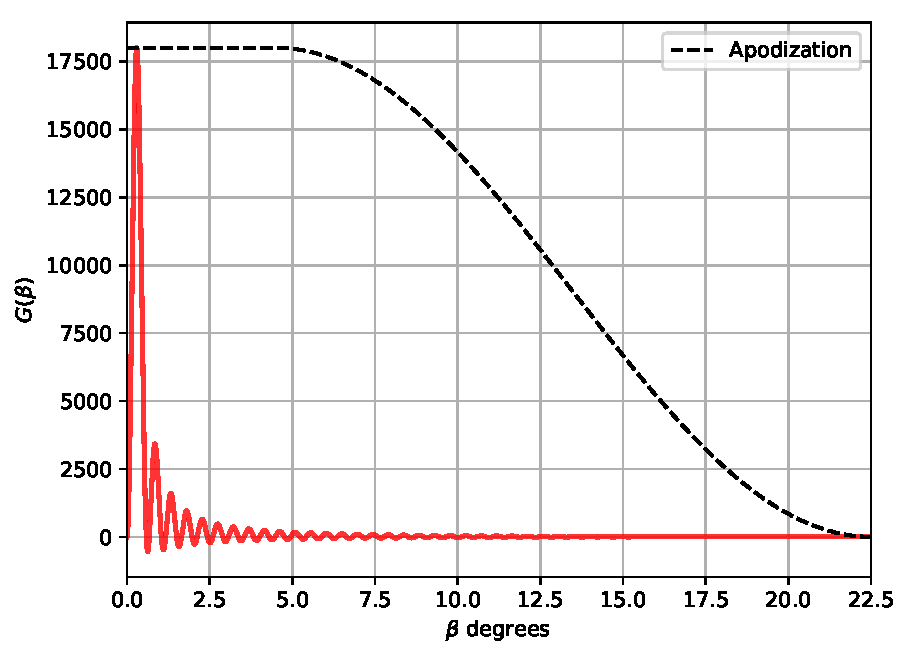
\includegraphics[width=0.45\columnwidth]{modified_radial_kernel.pdf}}
\subfigure[\label{fig:gl}]{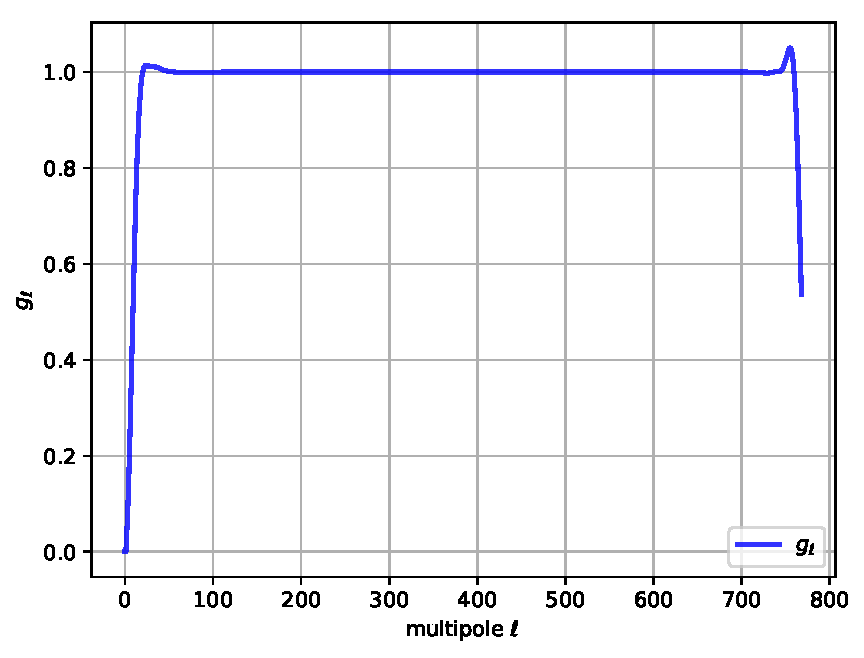
\includegraphics[width=0.45\columnwidth]{effective_beam.pdf}}
\caption{}
%\label{fig:rad_ker_decay}
\end{figure}
%
For this exercise, we work at a Healpix resolution of ${\textrm Nside}=256$. We simulate CMB polarization map using power spectra computed with CAMB with fiducial cosmological parameters and B-modes corresponding to $r=0.001$. We evaluate the $E/B$ maps using real space kernels on a patch of $10 ^{\circ} \times 25^{\circ}$, centered at zero galactic latitude and the long axis of the patch aligned with the equator. 
%
\begin{figure}[h]
\centering
\subfigure[Real space B]{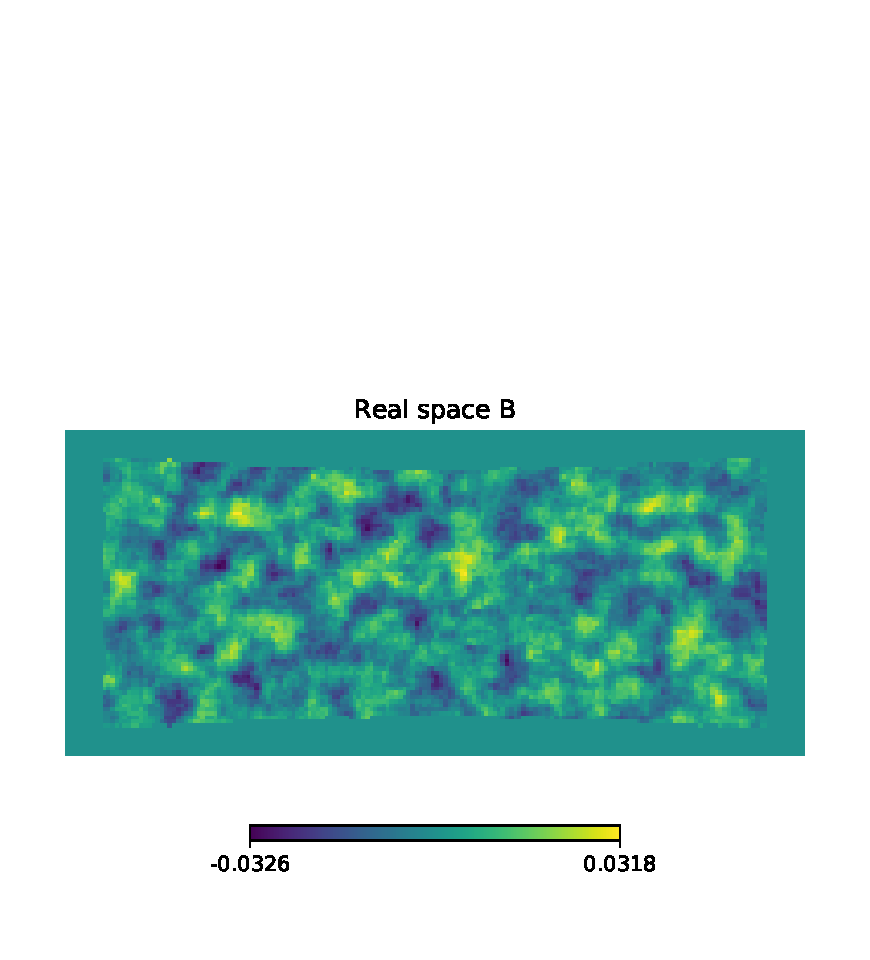
\includegraphics[width=0.45\columnwidth]{real_space_B.pdf}}
\subfigure[True B]{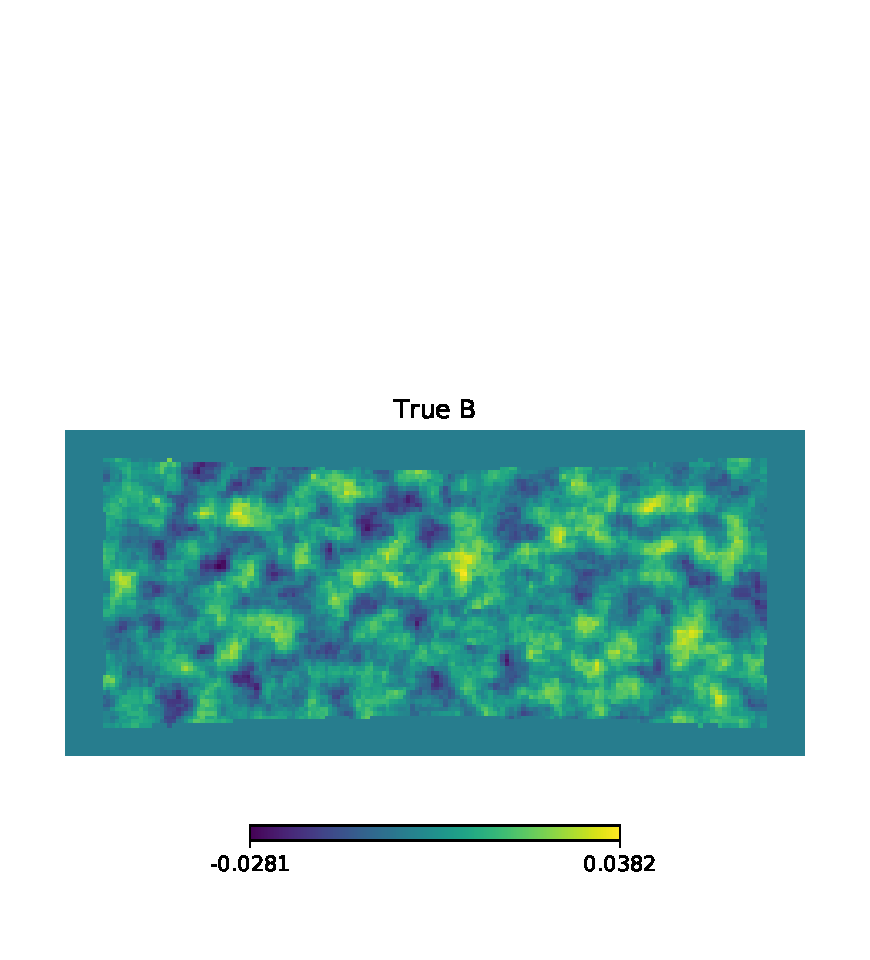
\includegraphics[width=0.45\columnwidth]{true_B.pdf}}
\caption{The figure on the left depicts the B-mode maps evaluated using the modified real space kernel while that on the right depicts the true B-mode map.}
\label{fig:compare_B}
\end{figure}
%
We evaluate the E/B maps using the real space operator, in which we modify the radial kernel by imposing a radial cut-off of $\sim 22^{\circ}$.  The radial kernel used for constructing the real space operator is shown in Fig. \ref{fig:fbeta} while the effective harmonic space filter corresponding to this radial filter is depicted in Fig.~\ref{fig:gl}. 

The resultant $B$ mode maps evaluated using the real space method and true B-mode map evaluated using the conventional method is shown in Fig~\ref{fig:compare_B}. 
%
\begin{figure}[!h]
\centering
\subfigure[E-mode power spectra]{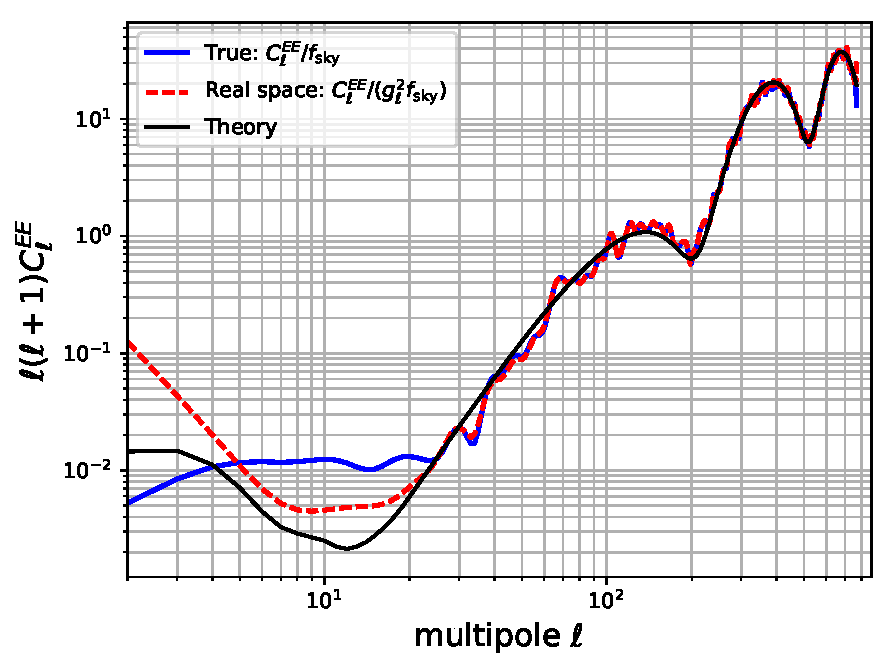
\includegraphics[width=0.45\columnwidth]{real_space_ee_spectra.pdf}}
\subfigure[B-mode power spectra]{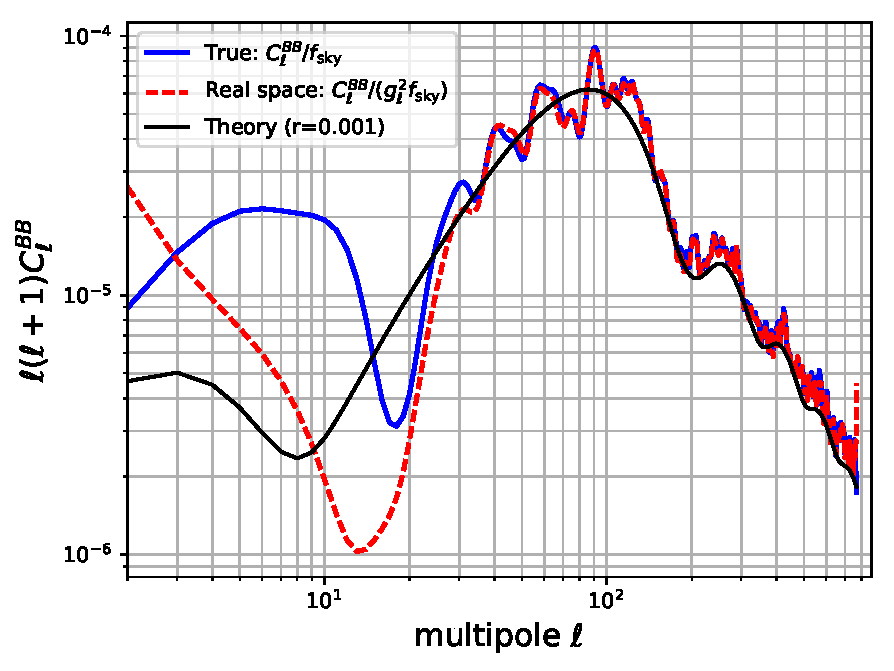
\includegraphics[width=0.45\columnwidth]{real_space_bb_spectra.pdf}}
\caption{In these plots, the black line depicts the theory power spectrum, the blue line depict the power spectrum evaluated from the true E/B maps while the red dashed lines depict the power spectrum evaluted from real space evaluated E/B maps.}
\label{fig:compare_spectra}
\end{figure}
%
Finally the power spectra estimated from $E/B$ maps evaluated using these real space operators and their comparison to the true power spectrum is depicted in Fig.~\ref{fig:compare_spectra}. 

Note that in the results presented here, we compute the $E/B$ maps on the square patch for which we have used Stokes parameters outside the mask boundary. Hence via the results presented here, we do not claim to address any issues relating to masking induced E/B mixing. However we would like to highlight the fact that using a modified radial kernel does not result in mixing of E/B power.

\end{document}
